\chapter{Implementation and Proposed Methodology}
\onehalfspacing

\section{System Overview}

The proposed framework for Hinglish multimodal sentiment analysis is built around two core contributions: the HinglishMSA dataset and the MulTHinglish model. The end-to-end system connects raw YouTube content on one end to a continuous sentiment score on the other, passing through five carefully engineered stages. Each stage introduces specific algorithmic choices that together address the unique challenges of code-mixed, resource-scarce, multilingual video data.

Figure~\ref{fig:tikz_pipeline} presents a high-level view of the complete processing pipeline.

\begin{figure}[ht]
\centering
\begin{tikzpicture}[
    node distance=0.35cm and 0.1cm,
    stg/.style={draw, fill=blue!9, minimum width=2.6cm, minimum height=1.1cm, align=center, font=\small},
    subs/.style={draw, fill=gray!7, minimum width=2.6cm, minimum height=0.55cm, align=center, font=\scriptsize},
    arr/.style={->, very thick, blue!60}
]
\node[stg] (s1) {\textbf{Stage 1}\\\scriptsize Data Collection};
\node[stg, right=0.55cm of s1] (s2) {\textbf{Stage 2}\\\scriptsize Preprocessing};
\node[stg, right=0.55cm of s2] (s3) {\textbf{Stage 3}\\\scriptsize Annotation};
\node[stg, right=0.55cm of s3] (s4) {\textbf{Stage 4}\\\scriptsize Feature Extr.};
\node[stg, right=0.55cm of s4] (s5) {\textbf{Stage 5}\\\scriptsize Model Train};

\node[subs, below=0.3cm of s1] {\scriptsize YouTube API\\1,174 videos};
\node[subs, below=0.3cm of s2] {\scriptsize Segmentation\\50,695 clips};
\node[subs, below=0.3cm of s3] {\scriptsize LLM Labels\\2,652 clips};
\node[subs, below=0.3cm of s4] {\scriptsize T+A+V\\vectors};
\node[subs, below=0.3cm of s5] {\scriptsize MulTHinglish\\regression};

\draw[arr] (s1)--(s2); \draw[arr] (s2)--(s3);
\draw[arr] (s3)--(s4); \draw[arr] (s4)--(s5);
\end{tikzpicture}
\caption{Five-stage HinglishMSA end-to-end pipeline from YouTube video collection to sentiment score prediction.}
\label{fig:tikz_pipeline}
\end{figure}

The five stages are: (1) \textbf{Dataset Construction} — collecting, segmenting, transcribing, and annotating Hinglish video clips from YouTube; (2) \textbf{Preprocessing and Filtering} — applying face detection, language identification, and quality filters to produce a clean, verified corpus; (3) \textbf{LLM-Assisted Annotation} — using a large language model via Groq API to assign continuous sentiment scores in $[-3, +3]$; (4) \textbf{Feature Extraction} — encoding each clip into fixed-dimensional representations using cross-lingual pre-trained encoders; and (5) \textbf{Model Training and Evaluation} — supervised regression with MulTHinglish under five experimental conditions. The remainder of this chapter describes each stage in detail.

\section{HinglishMSA Dataset Construction}

\subsection{Source Selection and Data Collection Strategy}

YouTube was selected as the primary data source for four reasons: (i) it hosts an enormous volume of informal Hinglish content from speakers across India; (ii) its Data API v3 provides structured programmatic access; (iii) its diversity of domains ensures the dataset captures naturally occurring sentiment variation rather than elicited speech; and (iv) unlike social media text, video content provides all three modalities — speech, visual, and text (via transcription) — from a single source.

Video collection was conducted using 25 targeted search queries spanning eight topic domains, designed to maximise speaker and sentiment diversity. Table~\ref{tab:queries} documents the domain categories and representative queries used.

\begin{table}[ht]
\centering
\caption{YouTube search query domains and example queries used for HinglishMSA collection}
\label{tab:queries}
\renewcommand{\arraystretch}{1.3}
\begin{tabular}{p{3.8cm} p{7.5cm}}
\toprule
\textbf{Domain} & \textbf{Representative Queries} \\
\midrule
Entertainment Reactions  & ``Hinglish vlog'', ``India daily life Hindi English'' \\
Movie / Series Reviews   & ``Bollywood review Hindi'', ``web series review Hinglish'' \\
Lifestyle Vlogs          & ``Hindi English conversation'', ``daily routine vlog'' \\
Product Unboxings        & ``unboxing Hindi English'', ``product review Hindi'' \\
Travel Vlogs             & ``travel vlog India Hindi'', ``trip experience Hindi'' \\
Educational Explainers   & ``topic explain Hinglish'', ``tutorial Hindi English'' \\
Opinion Commentary       & ``opinion video Hindi mix'', ``rant Hindi English'' \\
Social Commentary        & ``social issue Hindi'', ``current events Hinglish'' \\
\bottomrule
\end{tabular}
\end{table}

Each query was limited to 50 results with deduplication on video ID, returning 1,179 unique video IDs. For each video, the following metadata was logged: video ID, title, channel name, publication date, view count, and originating query. The collection was conducted over two days in early 2026 using a Python script that respects the API's quota limits (10,000 units/day).

\subsection{Download and Frame Extraction}

Audio streams were downloaded as 16\,kHz mono WAV files using \texttt{pytubefix}, a maintained Python wrapper for the YouTube download protocol. Concurrently, five temporally evenly-spaced JPEG key frames were extracted per video using \texttt{ffmpeg}'s seek operation. Key frame timestamps were computed as $t_i = i \cdot T / 6$ for $i \in \{1, 2, 3, 4, 5\}$, where $T$ is the total video duration in seconds. This uniform sampling strategy captures representative visual states throughout the video without requiring shot-boundary detection. A total of \textbf{1,174 out of 1,179 videos} were successfully downloaded; 5 videos failed due to regional content restrictions or post-collection removal.

\subsection{Audio Segmentation}

Full-length audio files (typically 5--30 minutes) were segmented into short utterance-level clips using \texttt{ffmpeg}'s silence detection filter (\texttt{silencedetect}). The filter computes a short-term RMS energy envelope over the audio and identifies boundaries where the energy drops below a threshold $\theta$ for a sustained duration $\delta$. The specific parameters used were:
\[
\theta = -35\,\text{dB}, \qquad \delta = 0.4\,\text{seconds}
\]

Clips were retained only if their duration $d$ satisfied $3 \leq d \leq 15$ seconds. Clips shorter than 3 seconds are unreliable for transcription and prosodic feature extraction; clips longer than 15 seconds frequently span multiple semantic utterances, violating the single-sentiment-per-clip assumption. This segmentation produced \textbf{50,695 clips} totalling approximately 19.65\,GB of audio data.

\subsection{Face Detection and Visual Filtering}

Since HinglishMSA targets sentiment expressed by visible on-screen speakers, clips without a detectable face are excluded. Face detection was applied to the five extracted JPEG frames per source video using OpenCV's Haar Cascade frontal face detector (\texttt{haarcascade\_frontalface\_default.xml}), which applies a sliding-window multi-scale detection algorithm originally proposed by Viola and Jones. A clip was marked as \textit{face-present} if at least one face was detected in at least one of the five frames. This conservative threshold prevents discarding clips in which the speaker is briefly off-screen.

Of 50,695 clips, \textbf{43,146 (85.3\%)} passed the face detection filter, indicating that the vast majority of collected content features on-screen speakers — consistent with the vlog and commentary genre of the source videos.

\subsection{Transcription with Whisper}

All face-present clips were transcribed using faster-whisper \cite{radford2023whisper} with the \texttt{large-v3} model. Faster-whisper is a reimplementation of Whisper using the CTranslate2 inference engine, which provides 4$\times$ faster inference than the reference PyTorch implementation at equivalent accuracy. The model was run on an NVIDIA RTX 4050 Laptop GPU (6.4\,GB VRAM) in CUDA float16 precision. Transcription parameters were set as follows: beam size = 5, language = ``hi'' (serving as a soft prior, not a hard constraint), and \texttt{word\_timestamps = True}.

Whisper performs per-segment language identification via its \texttt{detect\_language} mechanism, which conditions on a 30-second audio window. For code-mixed Hinglish speech, this single-label identification is unreliable: a clip containing 70\% Hindi and 30\% English words may be labelled as either language depending on which segments are phonetically dominant. A total of 29,500 out of 43,146 clips were successfully transcribed; the remainder were skipped due to CUDA out-of-memory errors on unusually long clips or audio files with corrupted headers.

\subsection{Hinglish Detection Algorithm}

Naive filtering using Whisper's per-segment language label identified only 1,019 clips (3.5\%) as Hinglish. This low recall is expected: Whisper's language identification assigns a single label per 30-second window and treats Hindi Romanisation as English. To substantially improve recall, a three-stage Hinglish detection algorithm was developed.

Figure~\ref{fig:tikz_detection} illustrates the decision flow of the algorithm.

\begin{figure}[ht]
\centering
\begin{tikzpicture}[
    node distance=0.4cm and 0.1cm,
    proc/.style={draw, fill=blue!8, minimum width=4.5cm, minimum height=0.65cm, align=center, font=\small},
    dec/.style={draw, fill=orange!12, minimum width=4.5cm, minimum height=0.65cm, align=center, font=\small},
    term/.style={draw, fill=green!12, minimum width=2.8cm, minimum height=0.55cm, align=center, font=\small},
    termr/.style={draw, fill=red!10, minimum width=2.8cm, minimum height=0.55cm, align=center, font=\small},
    arr/.style={->, thick}
]
\node[proc] (inp) {Input: Whisper Transcript};
\node[dec, below=0.45cm of inp] (s1) {Stage 1: Devanagari + Latin co-occur?};
\node[term, right=1.8cm of s1] (y1) {Hinglish};
\node[dec, below=0.45cm of s1] (s2) {Stage 2: Loanword lexicon match?};
\node[term, right=1.8cm of s2] (y2) {Hinglish};
\node[dec, below=0.45cm of s2] (s3) {Stage 3: $p_{\text{Hi}}>0.1$ AND $p_{\text{En}}>0.1$?};
\node[term, right=1.8cm of s3] (y3) {Hinglish};
\node[termr, below=0.45cm of s3] (rej) {Rejected};

\draw[arr] (inp)--(s1);
\draw[arr] (s1) -- node[above,font=\scriptsize]{Yes} (y1);
\draw[arr] (s1) -- node[right,font=\scriptsize]{No} (s2);
\draw[arr] (s2) -- node[above,font=\scriptsize]{Yes} (y2);
\draw[arr] (s2) -- node[right,font=\scriptsize]{No} (s3);
\draw[arr] (s3) -- node[above,font=\scriptsize]{Yes} (y3);
\draw[arr] (s3) -- node[right,font=\scriptsize]{No} (rej);
\end{tikzpicture}
\caption{Three-stage Hinglish detection algorithm. Stages are applied in order; a transcript exits the pipeline as soon as it satisfies any stage's criterion.}
\label{fig:tikz_detection}
\end{figure}

\begin{enumerate}
    \item \textbf{Script co-occurrence (Stage 1):} A transcript is classified as Hinglish if it contains at least one Devanagari character (Unicode range U+0900--U+097F) AND at least one Latin ASCII character, indicating genuine script-level code-mixing. This stage captures the most unambiguous instances with near-zero false positives.

    \item \textbf{English loanwords in Devanagari (Stage 2):} Common English loanwords rendered in Devanagari transliteration are detected using a curated lexicon. Transcripts containing both a recognised Devanagari loanword and Hindi-dominant context are accepted. This stage recovers cases where Whisper fully transcribed in Devanagari script despite the audio containing English-origin vocabulary.

    \item \textbf{Dual-language probability (Stage 3):} The \texttt{langdetect} library is applied to estimate per-language probability scores. A transcript where both Hindi and English posterior probabilities exceed a threshold $\tau$ is classified as Hinglish:
    \[
    \text{Hinglish} \Leftrightarrow p_{\text{Hindi}} > \tau \quad \text{AND} \quad p_{\text{English}} > \tau, \quad \tau = 0.10
    \]
    This stage recovers transcripts written entirely in Romanised script that mix Hindi words and English words without script-level cues.
\end{enumerate}

Applying this algorithm to the 29,500 transcriptions identified \textbf{6,740 Hinglish clips (22.8\%)} --- a $6.6\times$ improvement over naive language identification. The improvement demonstrates the inadequacy of single-label language detection for code-mixed content and motivates the multi-stage design.

\begin{figure}[htbp]
\centering
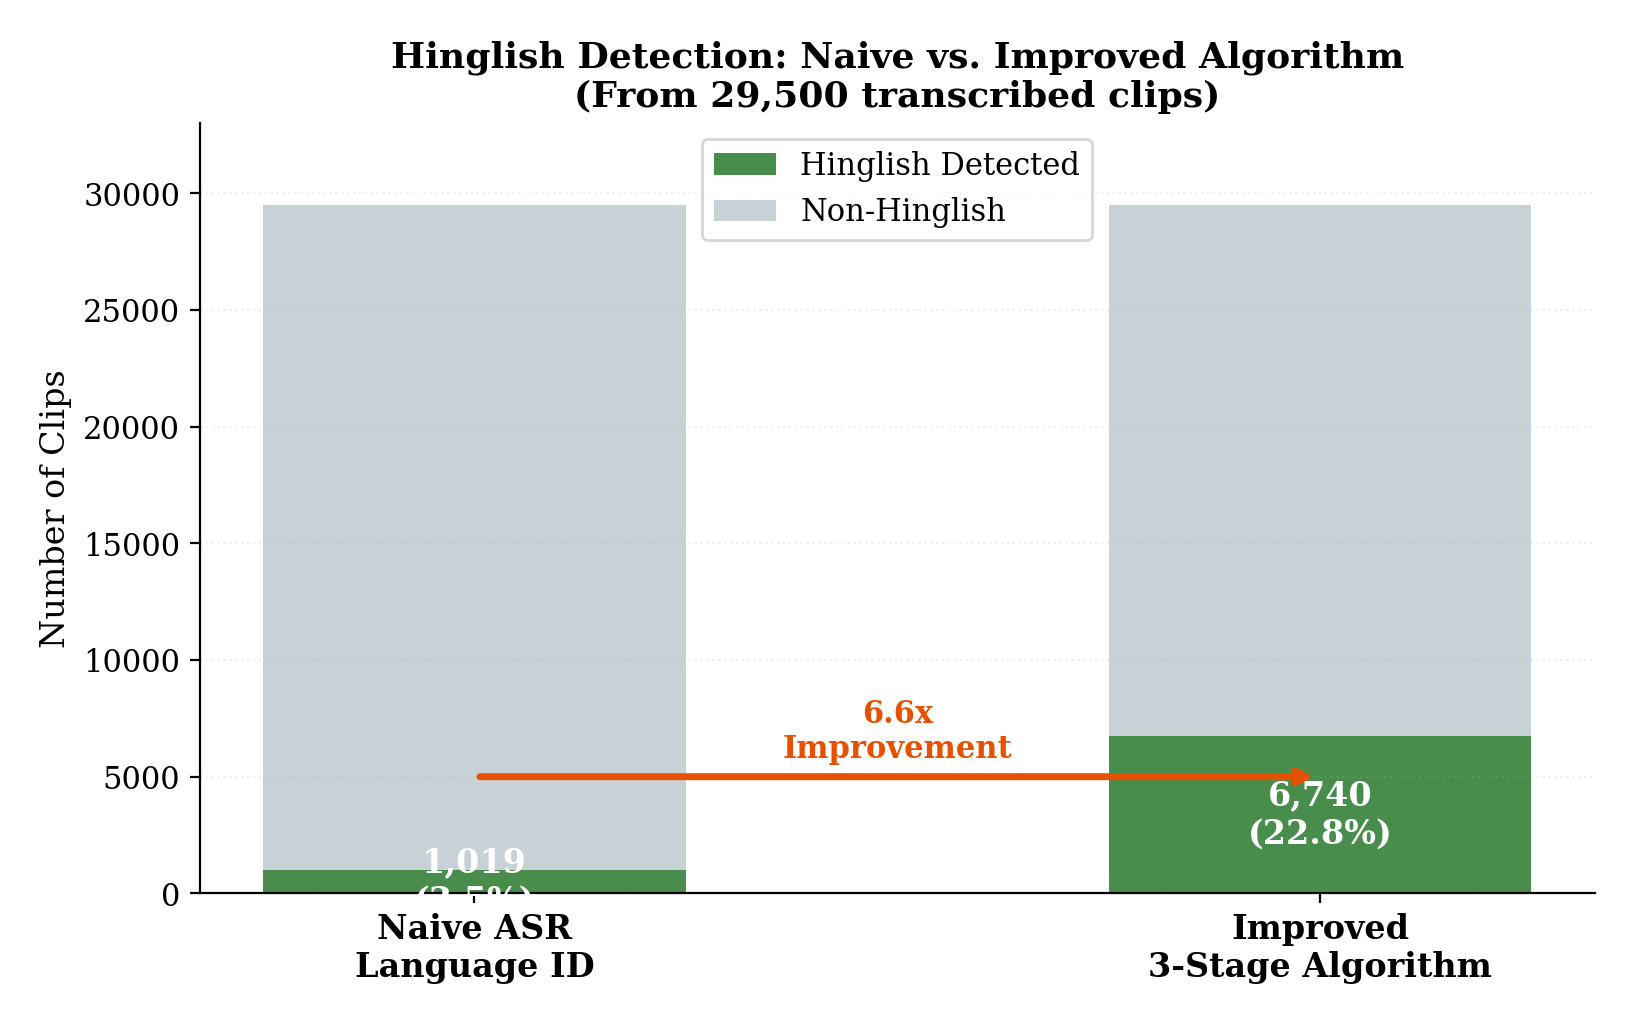
\includegraphics[width=0.78\textwidth]{./Figures/generated/fig_hinglish_detection}
\caption{Detection count comparison: naive ASR language label vs.\ three-stage Hinglish detection algorithm across 29,500 transcribed clips.}
\label{fig:detection}
\end{figure}

\subsection{LLM-Based Sentiment Annotation}

\subsubsection{Annotation Strategy}

Manual expert annotation of 6,740 clips by two bilingual annotators at 3 minutes per clip would require approximately 337 person-hours, making it economically and logistically infeasible in a research-scale project. To achieve scalable annotation, a pipeline was designed around the Groq inference API with the \texttt{llama\allowbreak-3.1\allowbreak-8b\allowbreak-instant} model, an 8-billion-parameter instruction-tuned language model optimised for low-latency inference.

Recent work has demonstrated that LLMs exhibit strong zero-shot sentiment understanding across languages, including code-mixed text, when provided with an explicit scale \cite{touvron2023llama}. The key advantage of this approach over crowdsourcing platforms (e.g., Amazon Mechanical Turk) is that it does not require a large pool of Hinglish-proficient annotators, which is a scarce and expensive resource for Indian language tasks.

\subsubsection{Prompt Design}

A minimal, direct prompt was designed to elicit continuous sentiment scores without requiring JSON parsing or complex output handling:

\begin{quote}
\texttt{Rate this Hinglish text sentiment: -3 (very negative) to +3 (very positive).\\
Return ONLY a single number like: -2.5 or 1.0 or 0\\
\\
Text: "\{text\}"\\
\\
Number:}
\end{quote}

The prompt specifies the rating scale explicitly and enforces a single-number response (\texttt{max\_tokens=10}), eliminating JSON parsing overhead. Temperature was set to $T=0.1$ for near-deterministic outputs, and a request timeout of 30 seconds was applied. API calls were serialised with a 0.1-second inter-request sleep to remain within the Groq free tier rate limit of 30 requests per minute.

\subsubsection{Confidence Stratification}

Since LLM annotations are inherently noisier for semantically ambiguous or near-neutral utterances, a confidence tier was assigned to each annotation based on the absolute magnitude of the predicted score $s$:
\begin{itemize}
    \item \textbf{High confidence} ($|s| \geq 1.5$): Strong polarity; the LLM expresses clear sentiment. Included in training and evaluation.
    \item \textbf{Medium confidence} ($0.5 \leq |s| < 1.5$): Moderate polarity; suitable for training but noisier. Included in training only.
    \item \textbf{Low confidence} ($|s| < 0.5$): Near-neutral; the clip may be factual speech, or the model may be uncertain. Excluded from all splits.
\end{itemize}

This stratification scheme mirrors the confidence-based filtering used in weakly-supervised NLP pipelines \cite{brown2020gpt3} and prevents noisy near-neutral annotations from biasing the regression objective.

\subsubsection{Annotation Results}

The pipeline processed 4,200 clips in approximately two hours. After removing entries with API failures (timeouts, malformed responses), \textbf{2,652 usable annotations} were retained. Of these:

\begin{itemize}
    \item High confidence: 1,498 clips ($|s| \geq 1.5$)
    \item Medium confidence: 1,103 clips ($0.5 \leq |s| < 1.5$)
    \item Low confidence (excluded): 51 clips ($|s| < 0.5$)
\end{itemize}

Sentiment score statistics: mean $= 0.02$ (approximately centred), standard deviation $= 1.54$, range $[-3.0, +3.0]$, with 1,497 negative-polarity clips ($s \leq 0$, 56.5\%) and 1,155 positive-polarity clips ($s > 0$, 43.5\%).

\subsection{Test Set Construction}

A held-out test set of \textbf{150 clips} was sampled from the high- and medium-confidence annotations using stratified random sampling (random seed = 42) with stratification bins defined at one-unit intervals across $[-3, +3]$. This ensures polarity and intensity balance in the test set, preventing evaluation bias towards a specific score range. The 150 clips were manually reviewed by the thesis author, who verified that the Groq-assigned sentiment scores were directionally consistent with the Hinglish text content. The remaining 2,501 clips constitute the training and validation pool.

\subsection{Dataset Statistics}

Table~\ref{tab:dataset_stats} presents the complete statistics of HinglishMSA.

\begin{table}[ht]
\centering
\caption{HinglishMSA dataset statistics across all pipeline stages}
\label{tab:dataset_stats}
\renewcommand{\arraystretch}{1.3}
\begin{tabular}{lr}
\toprule
\textbf{Statistic} & \textbf{Value} \\
\midrule
Source videos downloaded          & 1,174 \\
Total audio clips (all)           & 50,695 \\
Clips with face detected          & 43,146 (85.3\%) \\
Clips transcribed by Whisper      & 29,500 \\
Hinglish clips detected           & 6,740 (22.8\%) \\
\midrule
Total usable annotations          & 2,652 \\
\quad High confidence ($|s| \geq 1.5$)            & 1,498 \\
\quad Medium confidence ($0.5 \leq |s| < 1.5$)   & 1,103 \\
Training set                      & 2,251 \\
Validation set                    & 251 \\
Test set (human-verified)         & 150 \\
\midrule
Sentiment score mean              & 0.02 \\
Sentiment score std               & 1.54 \\
Negative clips ($s \leq 0$)       & 1,497 (56.5\%) \\
Positive clips ($s > 0$)          & 1,155 (43.5\%) \\
Score range                       & $[-3.0,\,+3.0]$ \\
\bottomrule
\end{tabular}
\end{table}

\begin{figure}[htbp]
\centering
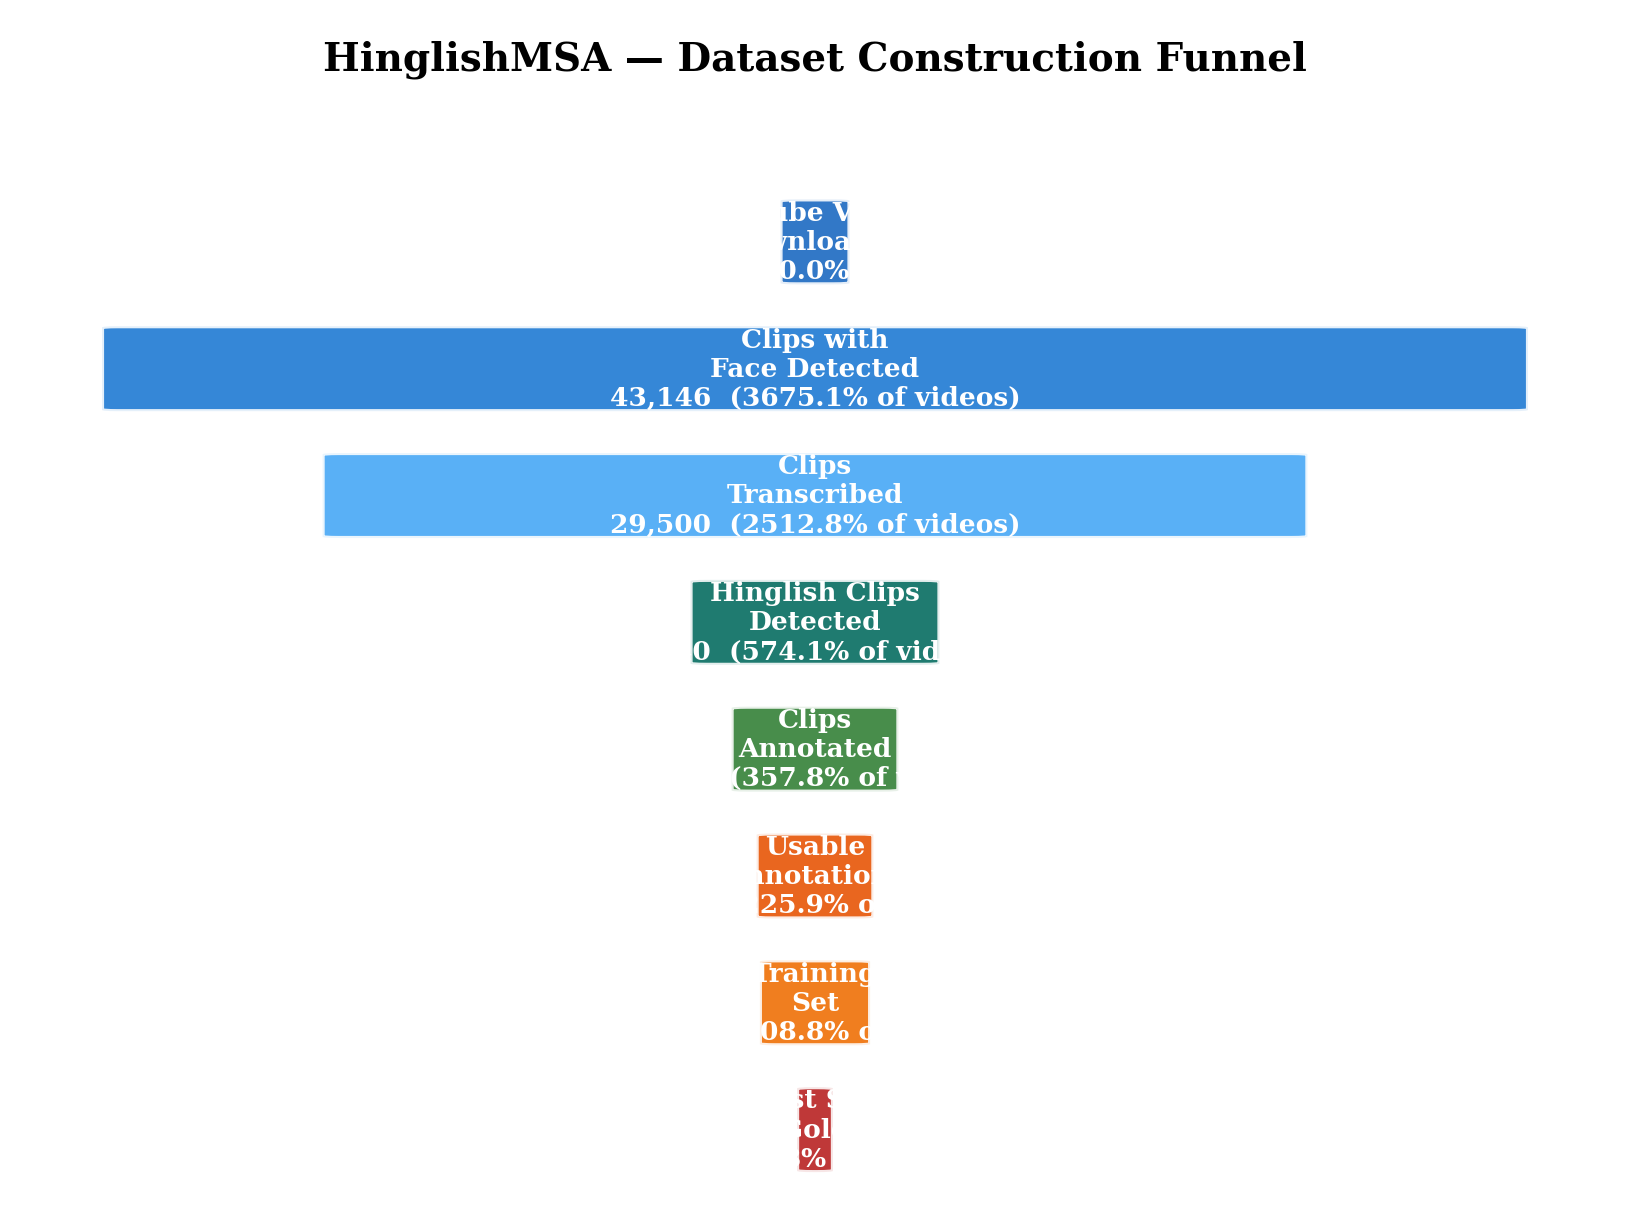
\includegraphics[width=0.72\textwidth]{./Figures/generated/fig_dataset_funnel}
\caption{HinglishMSA dataset construction funnel showing the number of clips surviving each filtering stage.}
\label{fig:funnel}
\end{figure}

\begin{figure}[htbp]
\centering
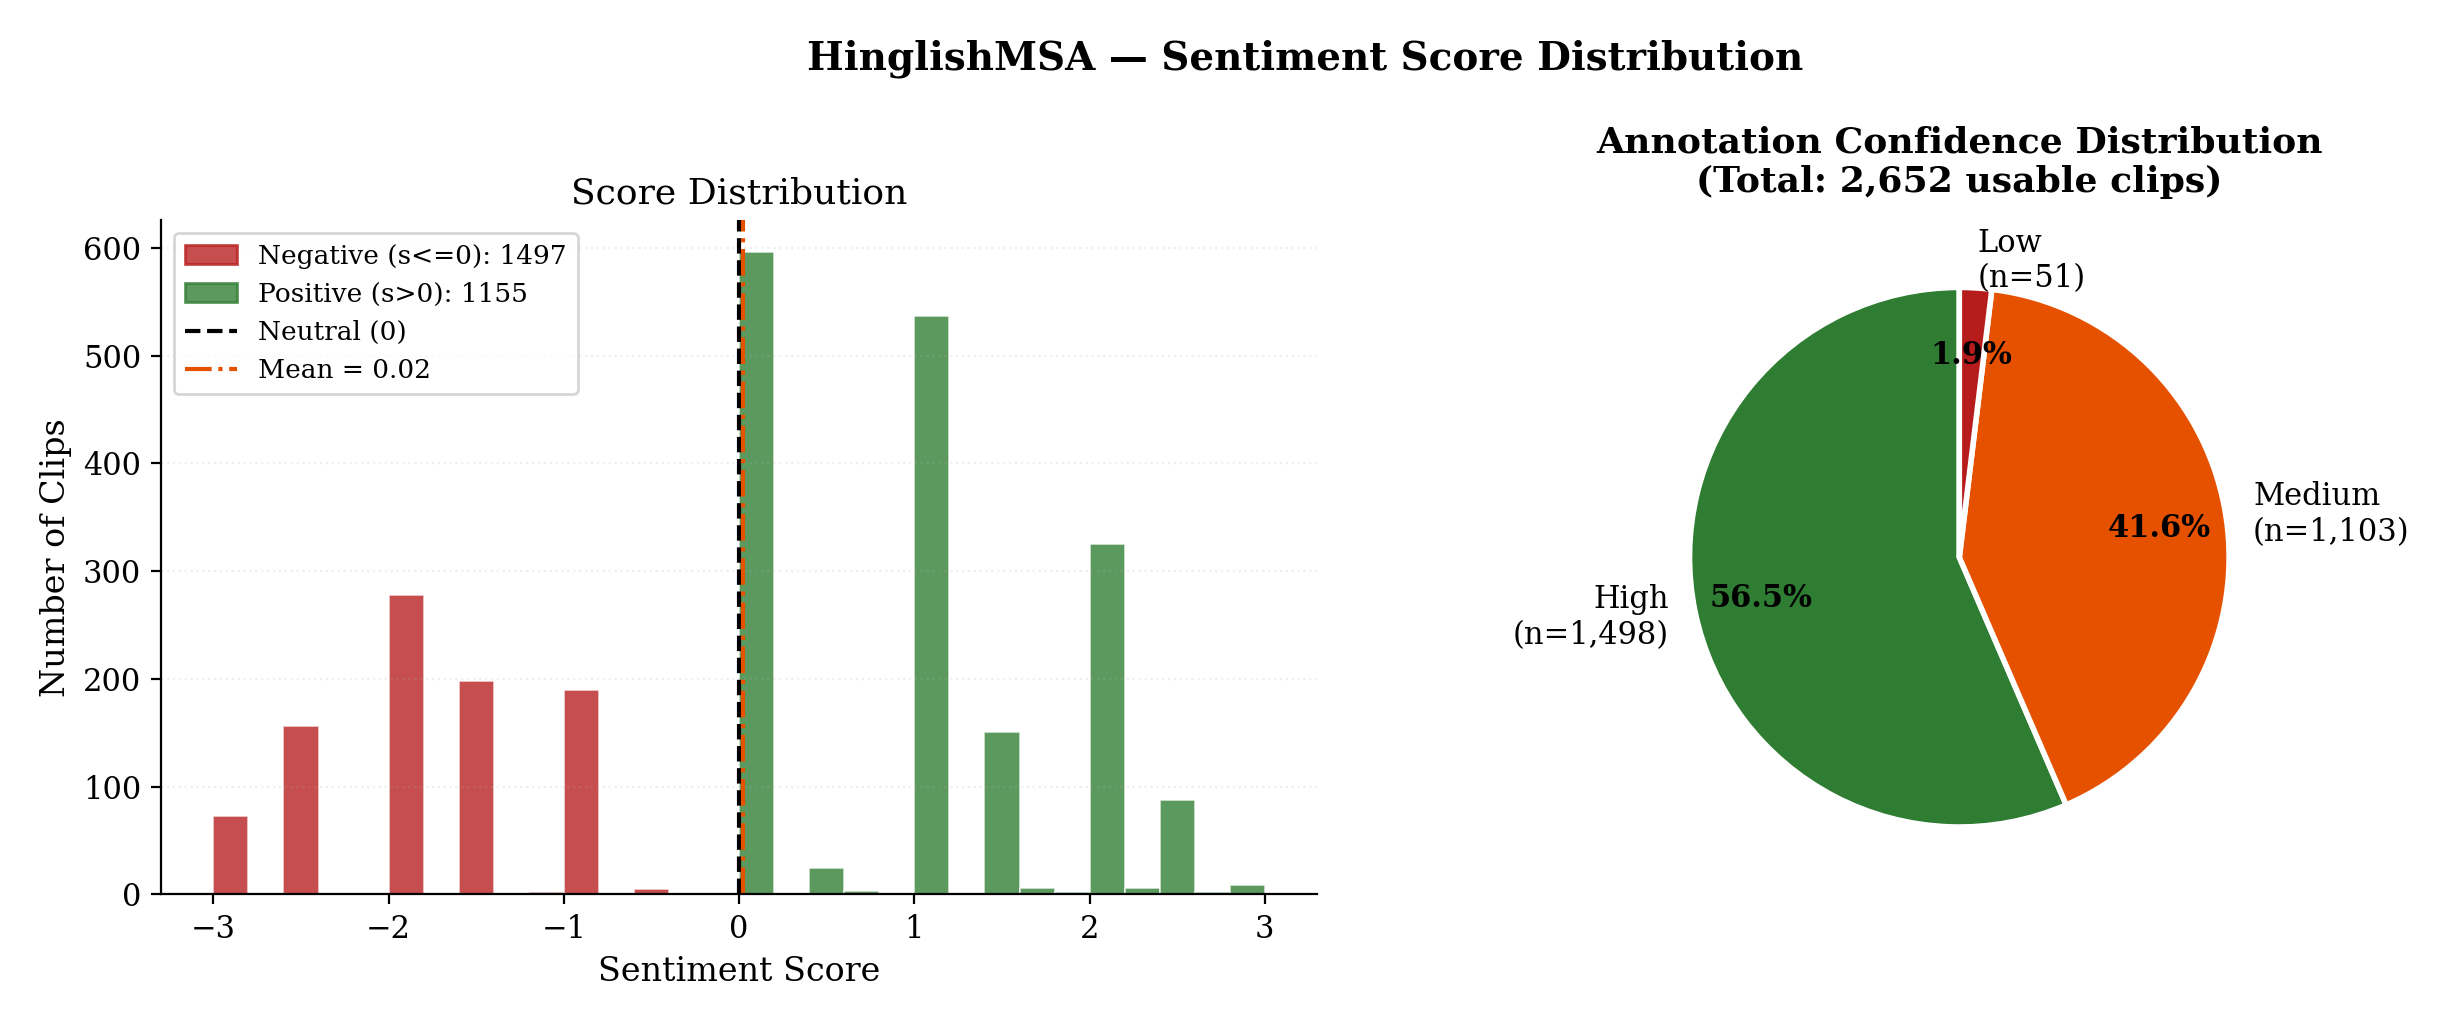
\includegraphics[width=\textwidth]{./Figures/generated/fig_score_distribution}
\caption{HinglishMSA sentiment score distribution (left) and annotation confidence breakdown (right).}
\label{fig:scoredist}
\end{figure}

\section{Feature Extraction}

Each annotated clip is represented as a triple $(\mathbf{t}, \mathbf{a}, \mathbf{v})$ where $\mathbf{t} \in \mathbb{R}^{768}$, $\mathbf{a} \in \mathbb{R}^{1024}$, and $\mathbf{v} \in \mathbb{R}^{512}$ are the text, audio, and visual feature vectors respectively. Features are extracted offline in a single pass before training and saved as NumPy arrays for efficient batched loading. Table~\ref{tab:features} summarises the three extraction pathways.

\begin{table}[ht]
\centering
\caption{Summary of feature extraction configuration for all three modalities}
\label{tab:features}
\renewcommand{\arraystretch}{1.3}
\begin{tabular}{llllll}
\toprule
\textbf{Modality} & \textbf{Model} & \textbf{Dim} & \textbf{Input} & \textbf{Pooling} & \textbf{Time} \\
\midrule
Text    & MuRIL-base \cite{khanuja2021muril}         & 768   & Token seq (max 128) & [CLS] token    & $\sim$15\,min \\
Audio   & wav2vec2-XLSR-53 \cite{conneau2021xlsr}    & 1024  & 16\,kHz waveform    & Temporal mean  & $\sim$40\,min \\
Visual  & CLIP ViT-B/32 \cite{radford2021clip}       & 512   & $224\times224$ JPEG & Frame mean     & $\sim$20\,min \\
\bottomrule
\end{tabular}
\end{table}

\subsection{Text Features: MuRIL}

Text features are extracted using MuRIL \cite{khanuja2021muril} (\texttt{google/muril-base-cased}), a 12-layer, 768-hidden-dimension BERT architecture pre-trained on 17 Indian languages plus their transliterated forms. The Whisper transcription for each clip is tokenised using MuRIL's SentencePiece vocabulary with a maximum length of 128 sub-word tokens; longer transcriptions are truncated and shorter ones are padded. Processing is conducted in batches of 32 on the RTX 4050 GPU in float32 precision. The \textbf{768-dimensional [CLS] token embedding} from the final transformer layer is extracted and used as the clip's text representation. This token aggregates bidirectional contextual information over the entire transcription, making it well suited for sentence-level sentiment classification \cite{devlin2019bert}.

\subsection{Audio Features: wav2vec2-XLSR-53}

Audio features are extracted using wav2vec2-XLSR-53 \cite{conneau2021xlsr} (\texttt{facebook/wav2vec2-large-xlsr-53}). The model is loaded in float16 precision, reducing the VRAM footprint from approximately 1.2\,GB to 600\,MB and allowing it to coexist with the text and visual models in the RTX 4050's 6.4\,GB VRAM budget. A critical implementation detail: all float32 waveform inputs must be explicitly cast to float16 before the forward pass; passing float32 inputs to a float16 model on CUDA produces zero-valued outputs due to silent precision mismatch in the convolutional layers.

Each 16\,kHz waveform is processed by \texttt{Wav2Vec2FeatureExtractor} (zero-mean normalisation, no attention mask) and passed through the model. The \textbf{mean-pooled hidden state} across the temporal sequence dimension yields a 1024-dimensional embedding that captures multilingual prosodic and phonetic information. Extraction checkpoints are written every 500 clips for fault tolerance, producing the final file \texttt{features/audio\_wav2vec2.npy} of shape $(2652, 1024)$.

\subsection{Visual Features: CLIP}

Visual features are extracted using CLIP ViT-B/32 \cite{radford2021clip}. For each clip, the five JPEG key frames from the source video are loaded and preprocessed using CLIP's standard pipeline: resize to $224\times224$, convert to RGB, and apply ImageNet mean/std normalisation ($\mu = (0.481, 0.457, 0.408)$, $\sigma = (0.269, 0.261, 0.276)$). The ViT-B/32 visual encoder then maps each frame to a 512-dimensional patch embedding via a 12-layer Vision Transformer. The embeddings from all five frames are \textbf{mean-pooled}, producing a single visual feature vector per clip that represents the average facial expression and visual context across the video. Output file: \texttt{features/visual\_clip.npy} of shape $(2652, 512)$.

Figure~\ref{fig:tikz_feat} visualises the combined feature extraction pipeline with dimensionalities.

\begin{figure}[ht]
\centering
\begin{tikzpicture}[
    node distance=0.45cm and 0.6cm,
    src/.style={draw, fill=gray!8, minimum width=3.0cm, minimum height=0.6cm, align=center, font=\small},
    enc/.style={draw, fill=blue!10, minimum width=3.0cm, minimum height=0.6cm, align=center, font=\scriptsize},
    vec/.style={draw, fill=orange!12, minimum width=3.0cm, minimum height=0.6cm, align=center, font=\scriptsize\bfseries},
    arr/.style={->, thick}
]
% --- Text column ---
\node[src] (ts) {Whisper Transcript};
\node[enc, below=0.35cm of ts] (te) {MuRIL-base [CLS]};
\node[vec, below=0.35cm of te] (tv) {$\mathbf{t} \in \mathbb{R}^{768}$};

% --- Audio column ---
\node[src, right=0.6cm of ts] (as) {16\,kHz WAV};
\node[enc, below=0.35cm of as] (ae) {wav2vec2-XLSR};
\node[vec, below=0.35cm of ae] (av) {$\mathbf{a} \in \mathbb{R}^{1024}$};

% --- Visual column ---
\node[src, right=0.6cm of as] (vs) {5 JPEG Frames};
\node[enc, below=0.35cm of vs] (ve) {CLIP ViT-B/32};
\node[vec, below=0.35cm of ve] (vv) {$\mathbf{v} \in \mathbb{R}^{512}$};

\draw[arr] (ts)--(te); \draw[arr] (te)--(tv);
\draw[arr] (as)--(ae); \draw[arr] (ae)--(av);
\draw[arr] (vs)--(ve); \draw[arr] (ve)--(vv);
\end{tikzpicture}
\caption{Feature extraction for the three modalities. Each clip produces a fixed-length vector stored offline before model training.}
\label{fig:tikz_feat}
\end{figure}

\section{MulTHinglish Model Architecture}

MulTHinglish extends the Multimodal Transformer (MulT) \cite{tsai2019multimodal} by replacing its English-centric text encoder with cross-lingual pre-trained representations and adapting the architecture for utterance-level regression on Hinglish data. The full model is parameterised by 5,283,713 learnable weights.

\begin{figure}[htbp]
\centering
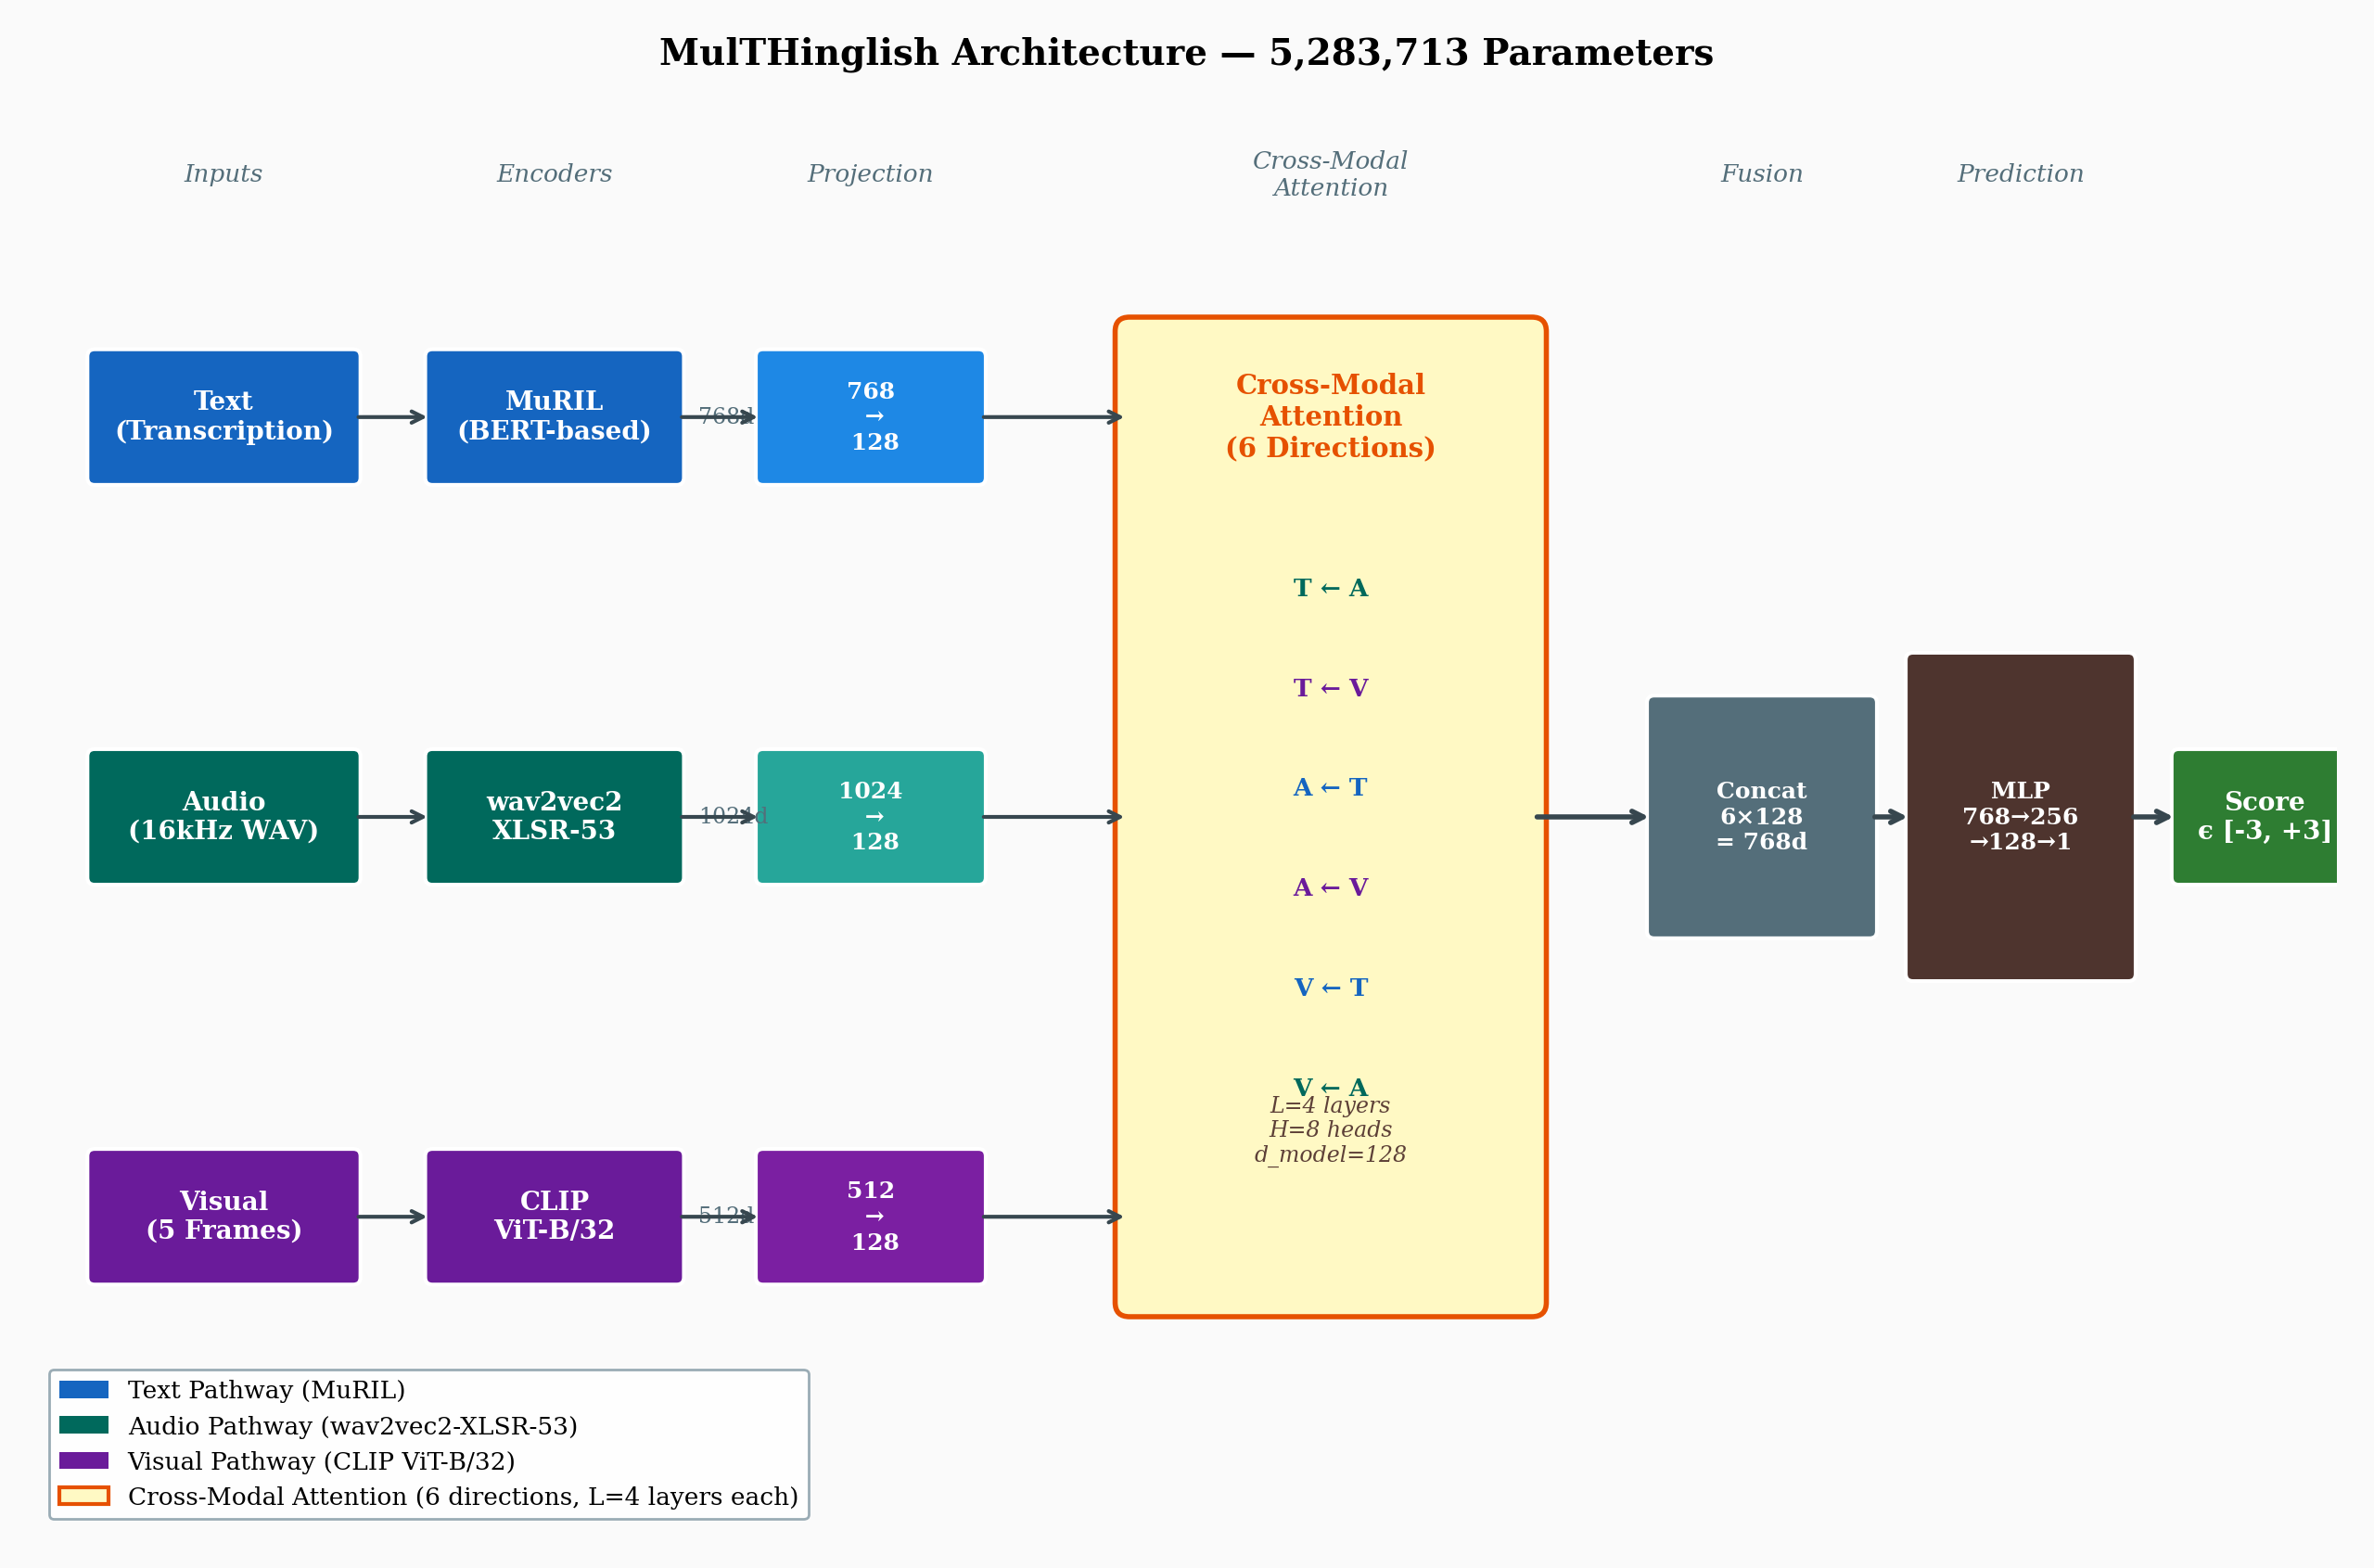
\includegraphics[width=\textwidth]{./Figures/generated/fig_multhilnglish_arch}
\caption{MulTHinglish architecture: three modality streams are projected to a common dimension, processed by six directed cross-modal attention modules, concatenated, and passed through a regression head.}
\label{fig:arch}
\end{figure}

\subsection{Modality Projection}

The three feature vectors arrive at different dimensionalities (768, 1024, 512) reflecting the architectural choices of their respective pre-trained encoders. A learned linear projection layer maps each to a common $d_{\text{model}} = 128$ dimensional space:
\[
\hat{\mathbf{t}} = W_t \mathbf{t} + b_t \in \mathbb{R}^{128}, \quad
\hat{\mathbf{a}} = W_a \mathbf{a} + b_a \in \mathbb{R}^{128}, \quad
\hat{\mathbf{v}} = W_v \mathbf{v} + b_v \in \mathbb{R}^{128}
\]
where $W_t \in \mathbb{R}^{128 \times 768}$, $W_a \in \mathbb{R}^{128 \times 1024}$, $W_v \in \mathbb{R}^{128 \times 512}$. The projection dimension $d_{\text{model}} = 128$ balances expressive capacity with computational efficiency given the relatively small dataset size. Projecting to a shared space also ensures that the cross-modal attention layers operate on representations of the same scale, preventing dominant modalities from saturating the attention softmax.

\subsection{Directional Cross-Modal Attention Layers}

For each ordered modality pair $(A \leftarrow B)$, a stack of $L = 4$ Cross-Modal Transformer (CMT) layers computes an attended representation of modality $A$ conditioned on information from modality $B$. Each CMT layer consists of:

\begin{enumerate}
    \item \textbf{Pre-layer normalisation:} LayerNorm is applied to both input representations before the attention operation. This pre-LN formulation yields more stable gradients than post-LN during training \cite{vaswani2017attention}.
    \item \textbf{Multi-head cross-modal attention} with $H = 8$ heads and key dimension $d_k = d_{\text{model}} / H = 16$:
    \[
    \text{CrossAttn}(A, B) = \text{softmax}\left(\frac{Q_A K_B^T}{\sqrt{d_k}}\right) V_B
    \]
    where $Q_A = W^Q \hat{a}$, $K_B = W^K \hat{b}$, $V_B = W^V \hat{b}$. The query comes from the modality being enriched ($A$) while the keys and values come from the modality providing context ($B$), realising a directional information flow from $B$ to $A$.
    \item \textbf{Position-wise feed-forward network:} Two linear layers with ReLU activation and hidden dimension $4 \cdot d_{\text{model}} = 512$, followed by a residual connection.
    \item \textbf{Residual connection and dropout:} Dropout at rate 0.1 applied after attention and after the FFN.
\end{enumerate}

The six directed cross-modal attention streams computed are:
\begin{itemize}
    \item $\mathbf{r}_{T \leftarrow A}$: text representation conditioned on audio context
    \item $\mathbf{r}_{T \leftarrow V}$: text representation conditioned on visual context
    \item $\mathbf{r}_{A \leftarrow T}$: audio representation conditioned on text context
    \item $\mathbf{r}_{A \leftarrow V}$: audio representation conditioned on visual context
    \item $\mathbf{r}_{V \leftarrow T}$: visual representation conditioned on text context
    \item $\mathbf{r}_{V \leftarrow A}$: visual representation conditioned on audio context
\end{itemize}

Each of the six ModuleLists contains $L = 4$ stacked layers, for a total of $6 \times 4 = 24$ cross-modal transformer layers.

\begin{figure}[htbp]
\centering
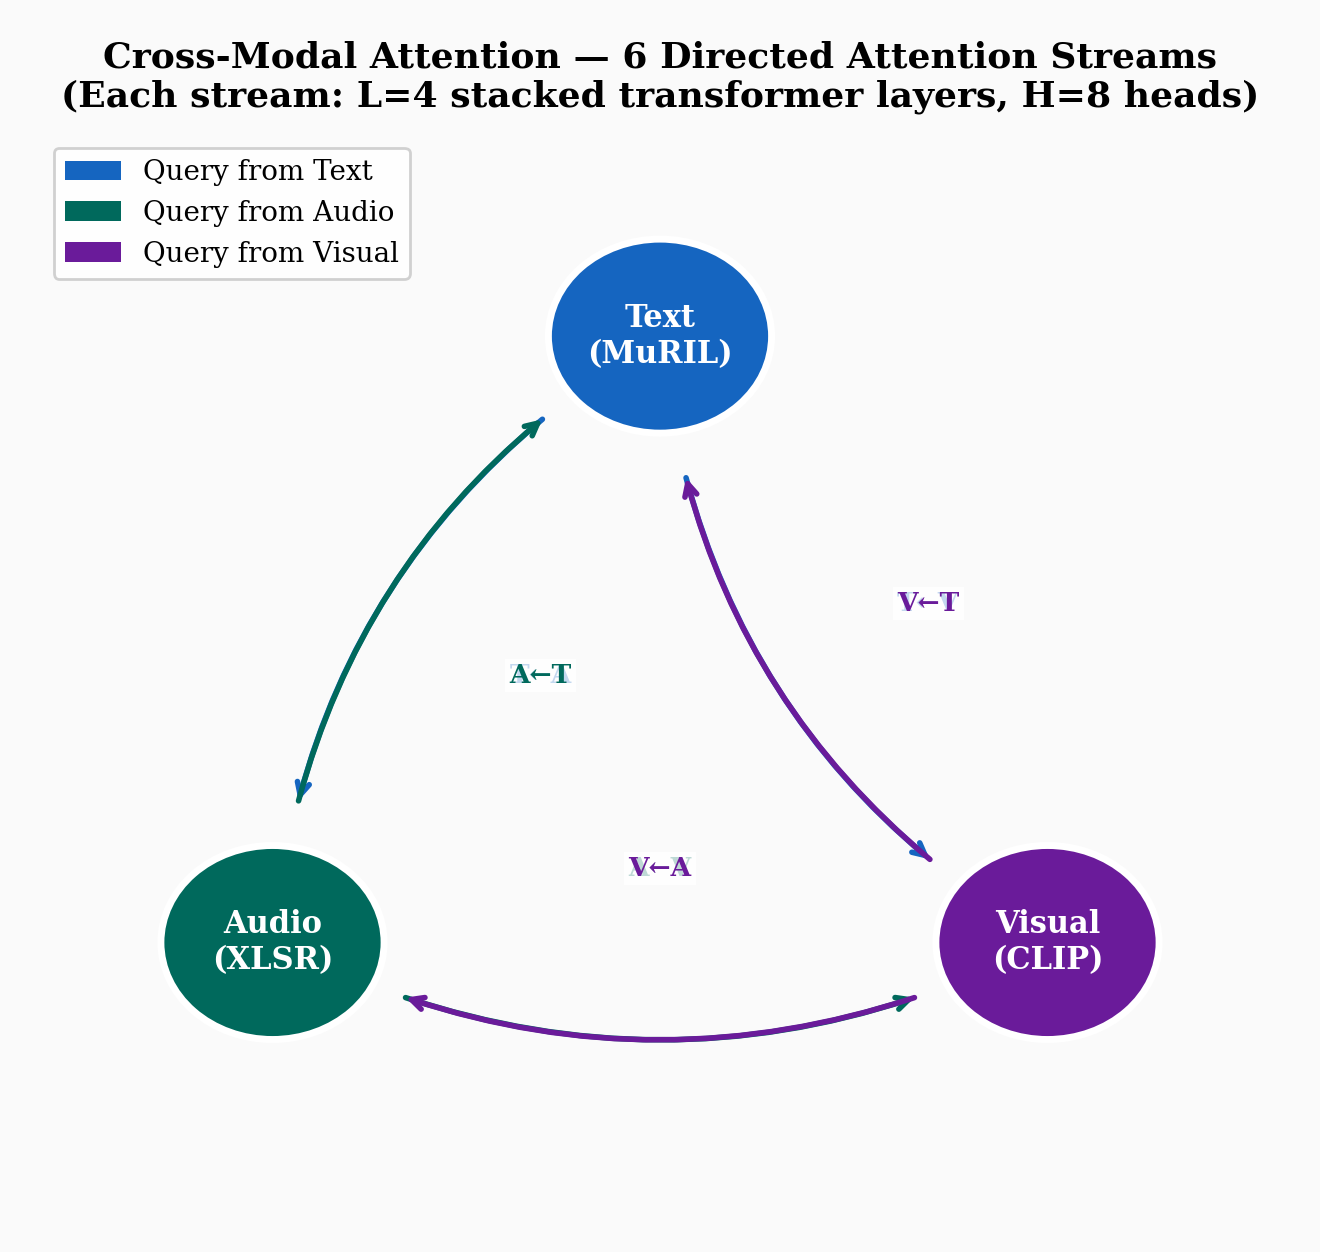
\includegraphics[width=0.62\textwidth]{./Figures/generated/fig_crossmodal_attention}
\caption{Six directed cross-modal attention streams in MulTHinglish (T = Text, A = Audio, V = Visual). Each directed edge represents a four-layer cross-modal transformer.}
\label{fig:crossattn}
\end{figure}

\subsection{Fusion and Prediction Head}

The six cross-modal attended representations are concatenated into a single $768$-dimensional fused vector ($6 \times 128 = 768$):
\[
\mathbf{z} = \text{Concat}(\mathbf{r}_{T \leftarrow A},\, \mathbf{r}_{T \leftarrow V},\, \mathbf{r}_{A \leftarrow T},\, \mathbf{r}_{A \leftarrow V},\, \mathbf{r}_{V \leftarrow T},\, \mathbf{r}_{V \leftarrow A}) \in \mathbb{R}^{768}
\]
This concatenation preserves the distinct contributions of all six cross-modal interactions rather than collapsing them into an average. The fused vector is then processed by a three-stage regression head:
\begin{align}
\mathbf{z}_1 &= \text{ReLU}(W_1 \mathbf{z} + b_1) \quad [768 \rightarrow 256] \\
\mathbf{z}_2 &= \text{ReLU}(W_2 \mathbf{z}_1 + b_2) \quad [256 \rightarrow 128] \\
\hat{y} &= W_3 \mathbf{z}_2 + b_3 \quad [128 \rightarrow 1]
\end{align}

The scalar output $\hat{y} \in \mathbb{R}$ is the predicted sentiment score. Dropout (rate 0.1) is applied before each linear transformation in the head to reduce overfitting on the relatively small dataset.

\subsection{Parameter Count Analysis}

Table~\ref{tab:params} breaks down the total parameter count by module to clarify where model capacity is concentrated.

\begin{table}[ht]
\centering
\caption{MulTHinglish parameter count breakdown by module}
\label{tab:params}
\renewcommand{\arraystretch}{1.3}
\begin{tabular}{lrr}
\toprule
\textbf{Module} & \textbf{Parameters} & \textbf{\% of Total} \\
\midrule
Input projection layers (3 linear) & 296,064 & 5.6\% \\
Cross-modal attention (6 streams $\times$ 4 layers) & 4,718,592 & 89.3\% \\
Regression head (3 linear layers) & 232,833 & 4.4\% \\
Layer normalisation (all LN layers) & 36,224 & 0.7\% \\
\midrule
\textbf{Total} & \textbf{5,283,713} & 100\% \\
\bottomrule
\end{tabular}
\end{table}

The cross-modal attention modules account for 89.3\% of model parameters, confirming that the representational budget is concentrated in the cross-modal interaction learning rather than the projection or head layers.

\section{Training Procedure}

\subsection{Data Splits}

From the 2,652 annotated clips, 150 clips are held out as the human-verified test set. The remaining 2,502 clips are split into training (2,251 clips, 90\%) and validation (251 clips, 10\%) using stratified random sampling with random seed 42. Stratification ensures that the sentiment score distribution in each split mirrors the overall distribution, preventing splits from being biased towards a specific polarity. Table~\ref{tab:splits} summarises the final split statistics.

\begin{table}[ht]
\centering
\caption{HinglishMSA train / validation / test split statistics}
\label{tab:splits}
\renewcommand{\arraystretch}{1.3}
\begin{tabular}{lccccc}
\toprule
\textbf{Split} & \textbf{Clips} & \textbf{Mean $s$} & \textbf{Std $s$} & \textbf{Neg (\%)} & \textbf{Pos (\%)} \\
\midrule
Training   & 2,251 & 0.02 & 1.54 & 56.4 & 43.6 \\
Validation &   251 & 0.03 & 1.53 & 56.6 & 43.4 \\
Test       &   150 & 0.01 & 1.55 & 56.7 & 43.3 \\
\bottomrule
\end{tabular}
\end{table}

\subsection{Optimisation Configuration}

Training uses the Adam optimiser \cite{vaswani2017attention} with an initial learning rate $\eta_0 = 10^{-3}$ and weight decay $\lambda = 10^{-4}$. Adam maintains per-parameter first and second moment estimates ($m_t$ and $v_t$):
\begin{align}
m_t &= \beta_1 m_{t-1} + (1 - \beta_1) g_t \\
v_t &= \beta_2 v_{t-1} + (1 - \beta_2) g_t^2 \\
\hat{m}_t &= m_t / (1 - \beta_1^t), \quad \hat{v}_t = v_t / (1 - \beta_2^t) \\
\theta_t &= \theta_{t-1} - \eta \cdot \hat{m}_t / (\sqrt{\hat{v}_t} + \epsilon)
\end{align}

with $\beta_1 = 0.9$, $\beta_2 = 0.999$, $\epsilon = 10^{-8}$. The loss function is mean squared error (MSE) over the training batch:
\[
\mathcal{L}_{\text{MSE}} = \frac{1}{N}\sum_{i=1}^{N}(y_i - \hat{y}_i)^2
\]

A ReduceLROnPlateau scheduler monitors the validation loss every epoch and halves the learning rate (factor = 0.5) if no improvement is observed for 5 consecutive epochs (patience = 5). Early stopping terminates training if validation loss does not improve for 15 consecutive epochs. The maximum number of training epochs is 100.

Gradient clipping with a maximum $L_2$ norm of 1.0 is applied before each parameter update to prevent gradient explosion during the early stages of cross-modal attention training. The best model checkpoint (lowest validation MSE) is saved and used for final test set evaluation.

\subsection{Training Infrastructure}

All experiments were conducted on a single NVIDIA GeForce RTX 4050 Laptop GPU (6.4\,GB GDDR6 VRAM) with CUDA 12.x and PyTorch 2.x. The training batch size was set to 64. Each epoch requires approximately 35 forward-backward passes over the training set. Total wall-clock training time per experiment was approximately 8--12 minutes. The full experimental suite (five configurations) was completed in under one hour on the same hardware.

\section{Experimental Configurations}

To systematically evaluate the contribution of each modality and the impact of the cross-lingual encoders, five experimental configurations were designed, each varying the input modalities or model type while holding the training procedure constant. Table~\ref{tab:experiments} summarises all five configurations.

\begin{table}[ht]
\centering
\caption{Five experimental configurations for ablation study of modality contributions}
\label{tab:experiments}
\renewcommand{\arraystretch}{1.35}
\begin{tabular}{clcccl}
\toprule
\textbf{Exp.} & \textbf{Name} & \textbf{Text} & \textbf{Audio} & \textbf{Visual} & \textbf{Purpose} \\
\midrule
E1 & Text-only (MuRIL)    & \checkmark & $\times$ & $\times$ & Unimodal text baseline \\
E2 & Audio-only (XLSR)    & $\times$ & \checkmark & $\times$ & Unimodal audio baseline \\
E3 & Visual-only (CLIP)   & $\times$ & $\times$ & \checkmark & Unimodal visual baseline \\
E4 & Bimodal (T+A)        & \checkmark & \checkmark & $\times$ & Text and audio fusion \\
E5 & Trimodal (T+A+V)     & \checkmark & \checkmark & \checkmark & Full MulTHinglish \\
\bottomrule
\end{tabular}
\end{table}

\textbf{E1 (Text-only)} serves as the primary unimodal baseline, using only MuRIL text features. This configuration quantifies the amount of sentiment information encoded in the Hinglish lexical content alone. \textbf{E2 (Audio-only)} and \textbf{E3 (Visual-only)} complete the unimodal baselines for the acoustic and visual channels. \textbf{E4 (Bimodal)} combines the two strongest modalities (text and audio, as expected from the MSA literature \cite{poria2017review}) to measure the complementary gain from prosodic features over text alone. \textbf{E5 (Trimodal)} is the full MulTHinglish model, which should achieve the highest performance if the visual channel carries non-redundant affect information. For the unimodal configurations (E1--E3), the cross-modal attention streams associated with the missing modalities are removed and the fusion concatenation is reduced accordingly.

Figure~\ref{fig:tikz_ablation} summarises the modality inclusion pattern across configurations.

\begin{figure}[ht]
\centering
\begin{tikzpicture}[
    node distance=0.2cm and 0.1cm,
    hdr/.style={draw, fill=blue!12, minimum width=1.5cm, minimum height=0.55cm, align=center, font=\small\bfseries},
    cel/.style={draw, fill=green!15, minimum width=1.5cm, minimum height=0.5cm, align=center, font=\small},
    emp/.style={draw, fill=red!8,   minimum width=1.5cm, minimum height=0.5cm, align=center, font=\small},
    lbl/.style={minimum width=2.8cm, align=right, font=\small}
]
% headers
\node[lbl] (h0) {Configuration};
\node[hdr, right=0.2cm of h0] (ht) {Text};
\node[hdr, right=0.1cm of ht] (ha) {Audio};
\node[hdr, right=0.1cm of ha] (hv) {Visual};

% E1
\node[lbl, below=0.2cm of h0] (r1) {E1 Text-only};
\node[cel, right=0.2cm of r1] (r1t) {\checkmark};
\node[emp, right=0.1cm of r1t] (r1a) {$\times$};
\node[emp, right=0.1cm of r1a] (r1v) {$\times$};

% E2
\node[lbl, below=0.15cm of r1] (r2) {E2 Audio-only};
\node[emp, right=0.2cm of r2] (r2t) {$\times$};
\node[cel, right=0.1cm of r2t] (r2a) {\checkmark};
\node[emp, right=0.1cm of r2a] (r2v) {$\times$};

% E3
\node[lbl, below=0.15cm of r2] (r3) {E3 Visual-only};
\node[emp, right=0.2cm of r3] (r3t) {$\times$};
\node[emp, right=0.1cm of r3t] (r3a) {$\times$};
\node[cel, right=0.1cm of r3a] (r3v) {\checkmark};

% E4
\node[lbl, below=0.15cm of r3] (r4) {E4 Text + Audio};
\node[cel, right=0.2cm of r4] (r4t) {\checkmark};
\node[cel, right=0.1cm of r4t] (r4a) {\checkmark};
\node[emp, right=0.1cm of r4a] (r4v) {$\times$};

% E5
\node[lbl, below=0.15cm of r4] (r5) {E5 Trimodal (full)};
\node[cel, right=0.2cm of r5] (r5t) {\checkmark};
\node[cel, right=0.1cm of r5t] (r5a) {\checkmark};
\node[cel, right=0.1cm of r5a] (r5v) {\checkmark};
\end{tikzpicture}
\caption{Modality inclusion matrix across the five experimental configurations. Green (\checkmark) indicates modality active; red ($\times$) indicates modality absent.}
\label{fig:tikz_ablation}
\end{figure}

\section{Implementation Details and Reproducibility}

\subsection{Software Stack}

The entire pipeline was implemented in Python 3.10. Key library versions are: PyTorch 2.1.0 (CUDA 12.1), Transformers 4.38.0 (Hugging Face), faster-whisper 0.10.0, OpenCV 4.9.0, \texttt{pytubefix} 5.3.0, NumPy 1.26.2, and scikit-learn 1.4.0. All random seeds (Python, NumPy, PyTorch) were fixed to 42 before every experiment.

\subsection{Reproducibility Measures}

To ensure reproducibility, the following measures were taken:
\begin{itemize}
    \item All feature files are stored as deterministic NumPy arrays; re-running extraction from the same audio/image inputs produces bit-identical outputs.
    \item The dataset split is fully determined by the random seed and stratification scheme documented in Section~3.2.8.
    \item Model weights at the best validation checkpoint are saved as \texttt{.pth} files together with the full training configuration in JSON format.
    \item The Groq API annotation step is the only non-deterministic component (due to external service state); the saved annotation CSV constitutes the ground truth for all reported experiments.
\end{itemize}

The project code and feature extraction scripts are available in the accompanying repository.

\newpage